\documentclass[english]{article}

\usepackage[utf8]{inputenc}
\usepackage{graphicx}
\usepackage[margin=2.5cm]{geometry}
\usepackage{eso-pic}
\usepackage{hyperref}
\usepackage{wrapfig}
\usepackage{lipsum}
\usepackage{array}
\usepackage{enumitem}
\usepackage{qtree}
\usepackage{color}
\usepackage{forest}
\usepackage{tikz}
\usepackage{grffile}
\usepackage{babel}
\usepackage{listings}
\usepackage{hyperref}
\hypersetup{
    colorlinks=true,
    linkcolor=blue,
    filecolor=magenta,      
    urlcolor=cyan,
}
 
\urlstyle{same}

\begin{document}
\begin{titlepage}
	\begin{center}
		\begin{figure}[t]
			\centering
			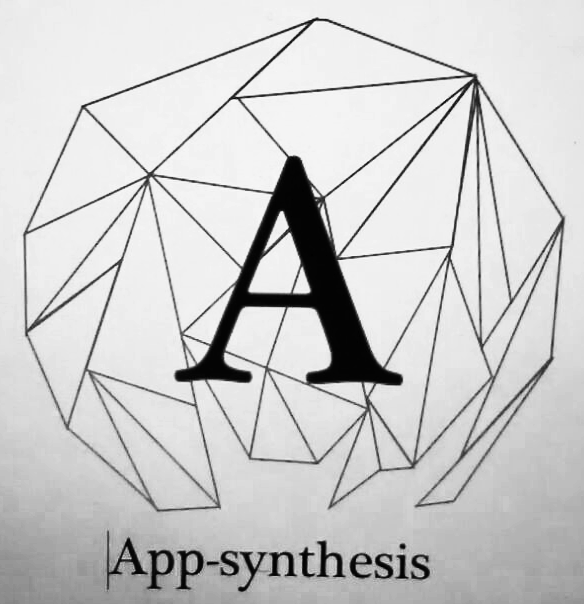
\includegraphics[width=350px]{logo.PNG}
		\end{figure}
		\begin{center}
			\textsc{\LARGE COS 301}
		\end{center}
		\begin{center}		
			\textsc{\LARGE V3D Graph Visualizer: User Manual}		
		\end{center}
		
		\begin{flushright} \large
			App-Synth \newline \emph{} \newline
		\end{flushright}


	\end{center}
\end{titlepage}

\tableofcontents
\newpage

\setcounter{page}{1}

\section{Introduction}
\subsection{System Overview}
This VDR3 graph is a graph visualization that allows users to perceive the information contained within digraphs which will be defined using the set of triples notations specified by Barla-Szabo in a 3D environment. The user should be able to change their vantage point while viewing the graph on a hyperplane or hypersphere.

\subsection{System Configuration}
Unity is used to create the VR system, whilst .cs code is used to create the Graph. Unity 2017.1 for development can run on Windows 7, 8 and 10 and also from MAC OS X 10.9 moving forward to later developments. For the development of the graph ideally Visual Studio can be used to debug .cs files. There are a few dependencies that are necessary for the functionality to be fully available.

\subsubsection{Dependency Requirements (Development)} 

\begin{itemize}
	\item \textbf{GPU}: Graphics card with DX9 (shader model 3.0) or DX11 with feature level 9.3 capabilities.
	\item \textbf{Visual Studio}: 2012 or higher. \href{https://www.visualstudio.com/downloads/}{Download Here}
	\item \textbf{Android Studio}: Android SDK and Java Development Kit (JDK) \href{https://developer.android.com/studio/index.html}{Download Here}
	
	\item \textbf{Internet Connection}: Desktop needs to have switched on its Wi-Fi to allow Mobile Server to connect to it as a hotspot.
	
\end{itemize}

\subsubsection{Dependency Requirements (Compiled App)}

\begin{itemize}
   \item A phone that runs Android 4.1 (Jelly Bean) or newer.
    
   \item Google Cardboard headset or similar
    
   \item 25mb minimum space to install the V3D app. 
\end{itemize} 


\section{Installation}
When One gets the executable apk on their mobile device, with a click on the apk, the android mobile device will install by initially requesting the user to grant access to the mobiles file system, so that the application can access the json files needed to load a graph. Once this has been established,the application will be installed onto the device. 

To run the Desktop version, the user would have needed to download the (.exe) file of the application. Once downloaded, User should run the application. 
\section{Getting Started}
Once you have installed all the dependencies and have launched the Application on both the Desktop application and the mobile application, you will be presented with the following interfaces:
\subsection{On Desktop}

\subsection{On Mobile}
        

\section{Usage} 
There could possibly exist some variance between which devices work with which versions of the headset, as well as which are fully compatible and which are only somewhat compatible \newline
\newline
Install and run the app.\newline From here, you can simply move your head to look freely around, in 360 degrees.

\section{Troubleshooting}

\end{document}
